%Matthias
\section{Use Case Diagramm}

\begin{figure}[H]
\centering
\centering
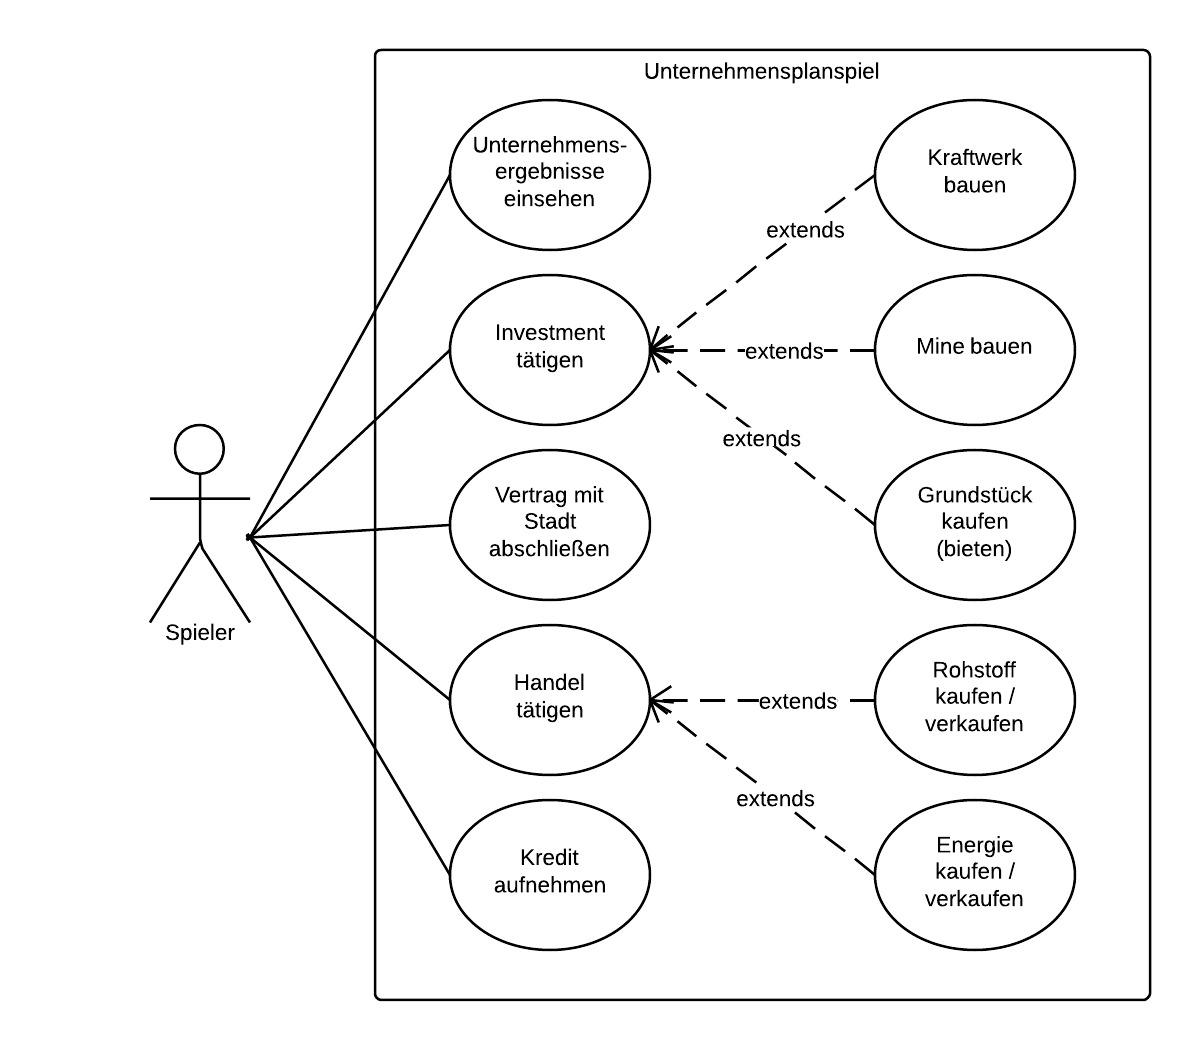
\includegraphics[width=0.9\textwidth]{se-wa-jpg/usecase}
\caption{Use Case Diagramm}
\label{Use Case Diagramm}
\end{figure}

Der Spieler hat im System des Unternehmensplanspiels folgende Optionen:
\begin{itemize}
  \item Investment t�tigen\\
  Hierunter fallen die folgenden Aktionen:
  	\begin{itemize}
  	  \item Mine bauen
  	  \item Kraftwerk bauen
  	  \item Grundst�ck kaufen
  	\end{itemize}
  \item Unternehmensergebnisse einsehen\\
  Der Spieler kann sich sowohl das Warenlager, den Kassenbestand, die Bilanz und
  die GuV einsehen.
  \item Vertrag mit Stadt abschlie�en\\
  Der Spieler kann mit St�dten einen Vertrag abschlie�en, um die Stadt mit
  Energie zu versorgen.
  \item Handel t�tigen\\
  Der Spieler kann die Rohstoffe Uran, Gas und Kohle zu Festpreisen kaufen oder
  verkaufen. Dar�ber hinaus kann er an der Energieb�rse �bersch�ssige Energie
  verkaufen oder fehlende Energie beziehen.
  \item Kredit aufnehmen
  Zur Finanzierung von Investitionen kann der Spieler einen Kredit aufnehmen.
  Die Konditionen sind dabei fest, der Spieler kann jedoch aus unterschiedlichen
  Krediten ausw�hlen.
\end{itemize}